\begin{figure}[H]
	\centering
	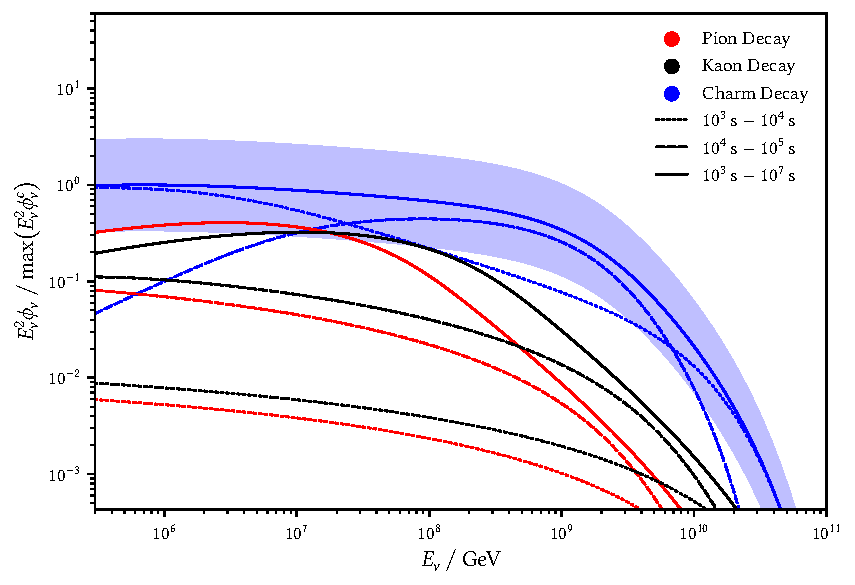
\includegraphics{../plots/build/magnetar_integrated_neutrino_spectrum_with.pdf}
	\caption[Magnetar $\nu \kern+0.5pt$ fluence compared to $c$ decay with optical depth.]
			{Expected neutrino fluence normalized to the maximum charm contribution from a~young magnetar for different time
			 intervals after formation, including the optical depth defined by \eqref{eqn:optical} as a modification.
			 Charmed hadrons dominate at all energies~except below $E_\nu = \kern-0.5pt \qty{e7}{\giga\electronvolt}$ for the
			 $\qty{e4}{\second} - \kern-1.0pt \qty{e5}{\second}$ integration. This is unexpected and therefore discussed further
			 in the text. The same shaded uncertainty band as in Figure \ref{fig:magnetar-flux-with} is adopted for charm decays.
			 Fluences are scaled by a factor $E_\nu^2$ for clarity and to facilitate the comparison to \cite{Carpio_2020}.}
	\label{fig:magnetar-fluence-with}
\end{figure}
